\documentclass{article}

% Language setting
% Replace `english' with e.g. `spanish' to change the document language
\usepackage[english]{babel}

% Set page size and margins
% Replace `letterpaper' with `a4paper' for UK/EU standard size
\usepackage[letterpaper,top=2cm,bottom=2cm,left=3cm,right=3cm,marginparwidth=1.75cm]{geometry}

% Useful packages
\usepackage{amsmath}
\usepackage{graphicx}
\usepackage[colorlinks=true, allcolors=blue]{hyperref}
\usepackage{braket} % Dirac notation packet
\usepackage{comment} % to comment large sections
\usepackage{mhchem} % left superscripts
\usepackage{subcaption} % use subfigures see: https://tex.stackexchange.com/questions/200994/environment-subfigure-undefined-on-journal-submission
\captionsetup{compatibility=false} % use subfigures

%%%%%%%%%%%%%%%%%%%%%%%%%%%%%%%%%%%%%%%%%%%%%%%%%%%
\usepackage{titlesec} % use paragraphs with numbers
\setcounter{secnumdepth}{4}
\titleformat{\paragraph}
{\normalfont\normalsize\bfseries}{\theparagraph}{1em}{}
\titlespacing*{\paragraph}
{0pt}{3.25ex plus 1ex minus .2ex}{1.5ex plus .2ex}
%%%%%%%%%%%%%%%%%%%%%%%%%%%%%%%%%%%%%%%%%%%%%%%%%%%

\title{Gravimeter with Magnetic Gradient}
\author{Edgar Zuniga}

\begin{document}
\maketitle

\begin{abstract}
Your abstract.
\end{abstract}

\section{Theoretical Framework}

\subsection{Condition for Atomic Interference within a Magnetic Gradient Field}
\subsubsection{Semi-classical Picture}

In this section, we review the condition needed to generate atomic interference in a gravimeter within a magnetic gradient. Let's consider an atom with total angular momentum number $F$. We will consider transitions between two stretch states with quantum magnetic number $m_{F}=\pm F$. Let's call the stretch state with $m_{F}=F$ as $\ket{1}$, and the stretch state with $m_{F}=-F$ as $\ket{2}$.

The atom is immersed inside a magnetic field of the following form

\begin{equation}\label{magnetic_field}
B = \eta z \hat{\textbf{z}}\
\end{equation}

where z is the position and $\eta$ is a constant with units of $[Tesla/meter]$. The atom will feel a force given by the gradient of the magnetic energy caused by the coupling of the total magnetic moment of the atom $\mu$ and the magnetic field, i.e.,

\begin{equation}\label{magnetic_force}
F = - \nabla (\pm \mu \eta z ) = \mp \mu \eta \
\end{equation}

Therefore, the atom will feel an acceleration due to the magnetic field proportional to its total magnetic moment. The total magnetic moment of the atom depends on its internal state, hence, the acceleration will depend on the hyperfine level under consideration. Let $a_m$ be the acceleration due to the magnetic gradient for the hyperfine state $\ket{1}$ and $-a_m$ the acceleration for the hyperfine state $\ket{2}$. Thus, the effective accelerations for state $\ket{1}$ and state $\ket{2}$ are respectively

\begin{equation}\label{a1}
a_{1} = -g + a_m
\end{equation}
\begin{equation}\label{a2}
a_{2} = -g - a_m
\end{equation}

where g is the acceleration due to gravity (taken to be positive), and $a_m$ is given by

\begin{equation}\label{am}
a_m = \mu \eta / m
\end{equation}

where $m$ is the mass of the atom under consideration.

In order to produce interference between these two states, we have to apply a $\frac{\pi}{2}$-pulse followed by a sequence of $\pi$-pulses and finally another $\frac{\pi}{2}$-pulse. The question that arises is, how many $\pi$-pulses do we need to apply in order to produce interference? To answer this question, we can picture a semi-classical approach where the interference condition is that the final position and the final velocity must coincide for both states.

\paragraph{Sequence of pulses $\frac{\pi}{2} - \pi - \frac{\pi}{2}$}
Let's study the classic sequence of pulses used to perform gravimetry and let's see if it can be used to obtain a signal for gravimetry in the presence of the magnetic force Eq.\ref{magnetic_force}.

Let $z_0$ and $v_0$ be the initial position and velocity respectively. The final velocity for each state is given respectively by the classical equation

\begin{equation}\label{v1_sequence_classic}
v_{1} = v_{0} + a_{1} T_{1} + a_{2} T_{2}
\end{equation}
\begin{equation}\label{v2_sequence_classic}
v_{2} = v_{0} + a_{2} T_{1} + a_{1} T_{2}
\end{equation}

where $T_{1}$ is the time elapsed between the first $\frac{\pi}{2}$-pulse and the $\pi$-pulse, and $T_{2}$ is the time elapsed between the $\pi$-pulse and the second $\frac{\pi}{2}$ pulse.

On the other hand, the final position for each state is given by the classical equation of motion

\begin{equation}\label{z1_sequence_classic}
z_{1} = (z_{0} + v_{0} T_{1} + \frac{a_{1} T^{2}_{1}}{2}) + (v_{0}+a_{1}T_{1})T_{2} + \frac{a_{2} T^{2}_{2}}{2}
\end{equation}
\begin{equation}\label{z2_sequence_classic}
z_{2} = (z_{0} + v_{0} T_{1} + \frac{a_{2} T^{2}_{1}}{2}) + (v_{0}+a_{2}T_{1})T_{2} + \frac{a_{1} T^{2}_{2}}{2}
\end{equation}

By using Eqs.\ref{v1_sequence_classic}-\ref{v2_sequence_classic}, and by demanding that the final velocities must be equal, we get that in order to produce interference, the acceleration $a_{1}$ must equal $a_{2}$ or alternatively, $T_{1}$ must equal $T_{2}$. Since, by assumption, $a_{1}$ and $a_{2}$ cannot be the same, then, the only acceptable condition is $T_{1}=T_{2}$. By accepting this condition on the duration of the pulses, and by using Eqs.\ref{z1_sequence_classic}-\ref{z2_sequence_classic} to demand that the final positions must be the same, we recover the unacceptable condition $a_{1}=a_{2}$. Therefore, we cannot produce interference in the presence of a magnetic force by applying just one $\pi$-pulse between the $\frac{\pi}{2}$ pulses.

\paragraph{Sequence of pulses $\frac{\pi}{2} - \pi - \pi - \frac{\pi}{2}$}

Let's study the sequence of pulses with an extra $\pi$-pulse before the last $\frac{\pi}{2}$-pulse. In this case, the equations for the final velocities are

\begin{equation}\label{final_v1}
v_{1} = v_{0} + a_{1} T_{1} + a_{2} T_{2} + a_{1} T_{3}
\end{equation}
\begin{equation}\label{final_v2}
v_{2} = v_{0} + a_{2} T_{1} + a_{1} T_{2} + a_{2} T_{3}
\end{equation}

Where $T_{3}$ is the time elapsed between the second $\pi$-pulse and the second $\frac{\pi}{2}$-pulse. Likewise, the equations for the final positions are

\begin{equation}\label{final_z1}
z_{1} = [(z_{0} + v_{0} T_{1} + \frac{a_{1} T^{2}_{1}}{2}) + (v_{0} + a_{1}T_{1})T_{2} + \frac{a_{2} T^{2}_{2}}{2}] + (v_{0}+a_{1}T_{1} + a_{2}T_{2})T_{3} + \frac{a_{1} T^{2}_{3}}{2}
\end{equation}
\begin{equation}\label{final_z2}
z_{2} = [(z_{0} + v_{0} T_{1} + \frac{a_{2} T^{2}_{1}}{2}) + (v_{0} + a_{2}T_{1})T_{2} + \frac{a_{1} T^{2}_{2}}{2}] + (v_{0}+a_{2}T_{1} + a_{1}T_{2})T_{3} + \frac{a_{2} T^{2}_{3}}{2}
\end{equation}

By using Eqs. (\ref{final_v1} and \ref{final_v2}) we get an equation that relates the periods between pulses as

\begin{equation}\label{times_relation}
T_{a} = 1 + T_{b}
\end{equation}

where we have defined $T_{a} \equiv \frac{T_{2}}{T_{1}}$ and $T_{b} \equiv \frac{T_{3}}{T_{1}}$. Now, by using Eqs. (\ref{final_z1} and \ref{final_z2}), and Eq. (\ref{times_relation}) we get the condition for the times elapsed between each pulse

\begin{equation}
\begin{aligned}
T_{2} = 2T_{1} \\
T_{1} = T_{3}
\end{aligned}
\end{equation}

These equations hold independently of the values for $a_{1}$ and $a_{2}$, as can be shown by substituting them into Eqs. (\ref{final_v1} and \ref{final_v2}). Therefore, the condition to get interference in the presence of a magnetic force is to apply a 
$\frac{\pi}{2}$-pulse followed by a $\pi$-pulse after a time $T$ has elapsed, then apply another $\pi$-pulse after a time $2T$ has elapsed, and finally, apply a $\frac{\pi}{2}$-pulse after a time $T$ elapsed, i.e., the sequence of pulses is

\begin{equation}\label{pulses}
\boldsymbol{\pi/2} \xrightarrow[]{T} \boldsymbol{\pi} \xrightarrow[]{2T} \boldsymbol{\pi} \xrightarrow[]{T} \boldsymbol{\pi/2}
\end{equation}

After the first $\frac{\pi}{2}$-pulse is applied, a superposition of states is created. In this semi-classical picture, each state moves independently with a different acceleration, that depends on the hyperfine levels under consideration and the magnitude of the gradient field at the position where each the state is located. Every time that a $\pi$-pulse is applied, the velocity of each state changes as shown in Fig. \ref{velocity_graph}. The final velocity for both states is the same as was required by the interference condition. Similarly, the final position for both states is the same just before the last $\frac{\pi}{2}$-pulse is applied in order to produce interference as can be seen in Fig. \ref{position_graph}. Interestingly, the position curves never cross each other during the lifetime of the superposition, unlike the velocity curves which cross each other once.

\begin{figure}
    \centering
    \begin{subfigure}{1\textwidth}
        \centering
        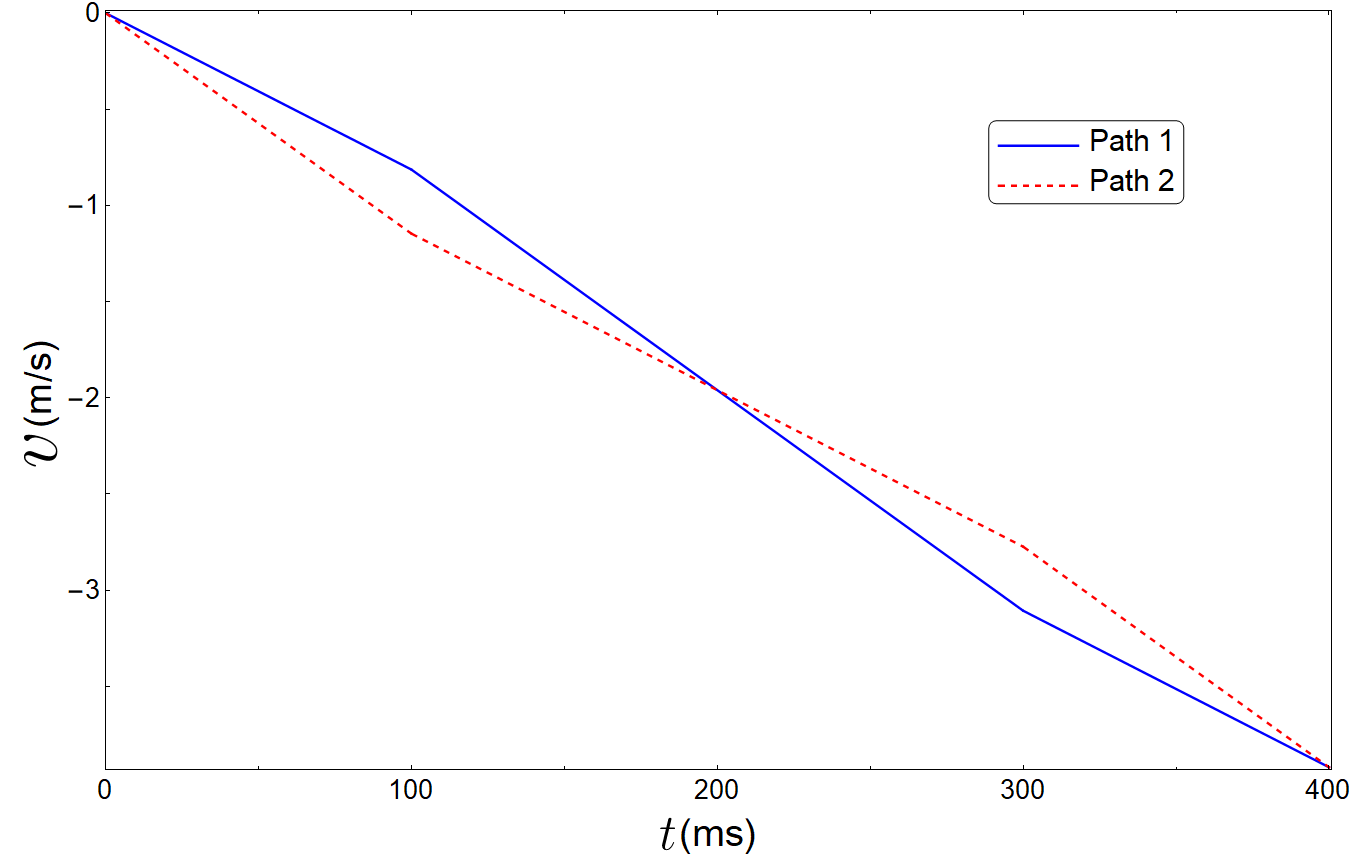
\includegraphics[width=0.8\textwidth]{velocidad.png}
        \caption{Velocity-time graph.}
        \label{velocity_graph}
    \end{subfigure}
    \hfill
    \begin{subfigure}{1\textwidth}
        \centering
        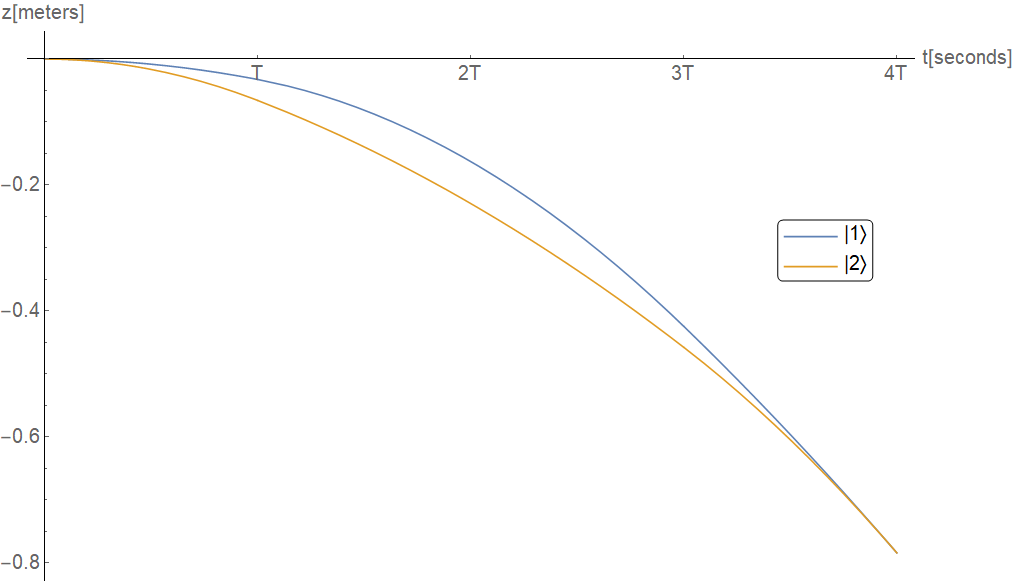
\includegraphics[width=0.8\textwidth]{posicion.png}
        \caption{Position-time graph.}
        \label{position_graph}
    \end{subfigure}
    \caption{Velocity and position vs. time graphs for each state after the superposition of hyperfine levels is created and just before they are made interfere. In these graphs $g=9.8m/s^2$, the mass $m$ is taken to be $87*1.6*10^{-27} Kg$ (approximately the mass of $\ce{^{87}_{}Rb}$), $\mu$ is taken to be the Bohr magneton with value $9.27*10^{-24} J/T$, $\eta$ has a value of $0.05 Tesla/meter$, and $T=100ms$. 
    The hyperfine state $\ket{1}$ has a quantum magnetic number of $m_{F}=F$ whereas the state $\ket{2}$ has a value of $m_{F}=-F$.}
    \label{velocity_position_graphs}
\end{figure}

\paragraph{Calculation of the Signal for Gravimetry}
Now that we have settled down the sequence of pulses needed to produce interference, we are in a position to compute the expected signal for gravimetry. In the semi-classical picture, each state of the superposition follows a different path and consequently accumulates a different phase. Therefore, to obtain the gravimetry signal, we need to compute the phase accumulated by each state during the lifetime of the superposition and then compute the difference between these two phases. 

The phase accumulated for each path is given by

\begin{equation}
\Phi = \int_{t_{0}}^{t} \omega(\ce{^{}_{}t{'}_{}})d\ce{^{}_{}t{'}_{}}
\end{equation}

where the angular frequency is given by the Planck relation $\omega = E / \hbar$, and the energy is given by the sum of the magnetic energy (Eq. \ref{magnetic_force}) and the energy due to the gravity field, i.e.,

\begin{equation}
E = \pm \mu B + mgz = (\pm \mu \eta + mg)z = C_{\pm} z
\end{equation}

where we have defined the constant $C_{\pm} \equiv \pm \mu \eta + mg$, with units of $[Joule/meter]$. Thus, accumulated phase will be given by

\begin{equation}\label{semi_classical_phase}
\Phi = \frac{C_{\pm}}{\hbar} \int_{t_{0}}^{t} z(\ce{^{}_{}t{'}_{}})d\ce{^{}_{}t{'}_{}}
\end{equation}

Each state's path is composed by three intervals $T_{1}=T$, $T_{2}=2T$, and $T_{3}=T$ (see Eq. \ref{pulses}). Thereby, for the first interval, the phase accumulated by each state will be respectively

\begin{equation}\label{phi1t1}
\Phi_{1, T_{1}} = \frac{C_{-}}{\hbar} \int_{0}^{T} (z_{0}+v_{0}t+a_{1} \frac{t^{2}}{2})dt
\end{equation}

\begin{equation}
\Phi_{2, T_{1}} = \frac{C_{+}}{\hbar} \int_{0}^{T} (z_{0}+v_{0}t+a_{2} \frac{t^{2}}{2})dt
\end{equation}

where $z_{0}$ and $v_{0}$ are respectively the initial position and velocity,
and the accelerations $a_{1}$ and $a_{2}$ are given by Eqs. \ref{a1} and \ref{a2}. The phase difference accumulated during the first interval is

\begin{equation}
\Delta \Phi_{T_{1}} = \Phi_{1, T_{1}} - \Phi_{2, T_{1}}
\end{equation}

Likewise, the phase accumulated during the second interval for each state is

\begin{equation}
\Phi_{1, T_{2}} = \frac{C_{+}}{\hbar} \int_{0}^{2T} [(z_{0}+v_{0}T+a_{1} \frac{T^{2}}{2}) + (v_{0}+a_{1}T)t + a_{2} \frac{t^{2}}{2}]dt
\end{equation}

\begin{equation}
\Phi_{2, T_{2}} = \frac{C_{-}}{\hbar} \int_{0}^{2T} [(z_{0}+v_{0}T+a_{2} \frac{T^{2}}{2}) + (v_{0}+a_{2}T)t + a_{1} \frac{t^{2}}{2}]dt
\end{equation}

The corresponding phase difference for this interval is

\begin{equation}
\Delta \Phi_{T_{2}} = \Phi_{1, T_{2}} - \Phi_{2, T_{2}}
\end{equation}

Finally, for the last interval, the phase accumulated by each state is

\begin{equation}
\Phi_{1, T_{3}} = \frac{C_{-}}{\hbar} \int_{0}^{T} [((z_{0}+v_{0}T+a_{1} \frac{T^{2}}{2}) + (v_{0}+a_{1}T)(2T) + a_{2} \frac{(2T)^{2}}{2}) + (v_{0}+a_{1}T + a_{2}(2T))t + a_{1} \frac{t^{2}}{2}]dt
\end{equation}

\begin{equation}
\Phi_{2, T_{3}} = \frac{C_{+}}{\hbar} \int_{0}^{T} [((z_{0}+v_{0}T+a_{2} \frac{T^{2}}{2}) + (v_{0}+a_{2}T)(2T) + a_{1} \frac{(2T)^{2}}{2}) + (v_{0}+a_{2}T + a_{1}(2T))t + a_{2} \frac{t^{2}}{2}]dt
\end{equation}

The phase difference accumulated during the last interval is

\begin{equation}\label{delphi3}
\Delta \Phi_{T_{3}} = \Phi_{1, T_{3}} - \Phi_{2, T_{3}}
\end{equation}

Therefore, by using Eqs.(\ref{a1}-\ref{a2} , and \ref{phi1t1}-\ref{delphi3}), the total phase difference accumulated during the three intervals is

\begin{equation}
\Delta \Phi = \Delta \Phi_{T_{1}} + \Delta \Phi_{T_{2}} + \Delta \Phi_{T_{3}} = 8 \frac{mga_{m}T^3}{\hbar}
\end{equation}

\begin{equation}\label{gravimetry_signal}
\Delta \Phi = 8 \frac{\mu \eta g T^3}{\hbar}
\end{equation}

where in the last equation we have used the definition of $a_m$ (Eq.\ref{am}). 

The Eq.\ref{gravimetry_signal} is the signal for gravimetry, which is proportional to $T^3$ and also proportional to the magnetic field via the constant $\eta$, these are the parameters we can adjust within a gravimetric experiment in order to increase the precision of the measurement. In Fig.\ref{phase_graph}, we can see the strong of the gravimetry signal for typical values of the constants in Eq.\ref{gravimetry_signal}. (\textcolor{red}{¿Ahora sí cuadran el cálculo teórico y el numérico del programa?})

\begin{figure}
\centering
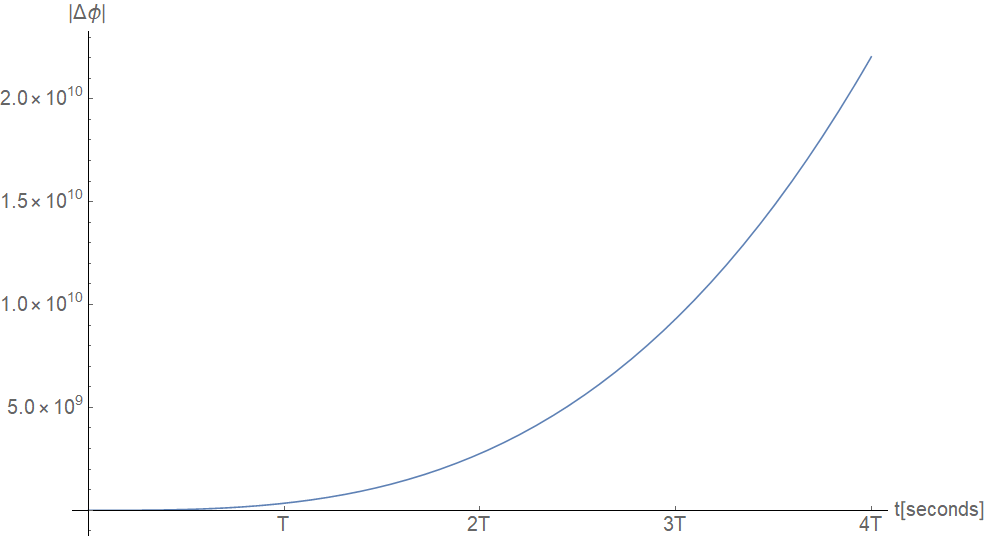
\includegraphics[width=0.9\textwidth]{fase.png}
\caption{Gravimetry signal for an atom falling down inside a linear magnetic field. This graph was obtained by using the same constant values as described in Fig.\ref{velocity_position_graphs}.}
\label{phase_graph}
\end{figure}

\subsubsection{Quantum Picture}
The calculations above were made by using a semi-classical picture to represent the superposition of states. Nevertheless, a correct calculation of the signal for gravimetry demands solving the Schrodinger equation for the evolution of each state in the superposition. 

In the following, we will consider a coherent wave packet of alkali-metal atoms with quantized center-of-mass motion along the z-axis, subject to a constant gravitational field and interacting with a classical magnetic field of the form given by Eq.\ref{magnetic_field}. The wave packet is given at time $t=0$ by

\begin{equation}\label{wave_packet}
\psi(z,0) = 
\left[\frac{1}{2 \pi (\Delta Z(0))^2} \right]^{1/4} \exp \left[-\frac{1}{4} \left[\frac{z-z_{0}}{\Delta Z(0)}\right]^{2}  + i \frac{p_{0}}{\hbar}z \right]
\end{equation}

where $z$ is the position coordinate, $\Delta Z(0)$ is the width of the wave packet centered at $z_{0}$, and $\frac{p_{0}}{\hbar}$ is the wave number of the wave packet. 

Before continuing, we introduce the non-dimensional position $x \equiv \kappa z$, and define the non-dimensional representation of this wave packet as

\begin{equation}\label{wave_packet_non_dimensional}
\phi(x,0) \equiv \frac{1}{\sqrt{\kappa}} \psi(\frac{x}{\kappa}, 0)
\end{equation}

where we have defined the inverse of the characteristic length of the system as

\begin{equation}\label{kappa}
\kappa \equiv (g_{s}\frac{\mu_{B}}{\hbar} + g_{n}\frac{\mu_{n}}{\hbar}) \frac{\eta}{\Delta W} > 0
\end{equation}

(\textcolor{red}{luego discutimos el significado de kapa, epsilon y otros símbolos de aquí.}) where $g_{s}$ is the electron spin $g$ factor, $g_{n}$ is the nuclear $g$ factor, $\mu_{B}$ is the Bohr magneton, $\mu_{n}$ is the nuclear magneton, $\hbar \Delta W$ is the field-free ground-state hyperfine splitting energy, and $\eta$ is the proportionality constant of the magnetic field (Eq.\ref{magnetic_field}).

The time-evolution of the non-dimensional wave packet (Eq.\ref{wave_packet_non_dimensional}) is given by (see \cite{Castanos2014} for additional details)

\begin{equation}\label{wave_packet_non_dimensional_evolution}
\phi(x,\tau) = 
\left[\frac{1}{2 \pi (\sigma_{x}(\tau))^2} \right]^{1/4} \exp \left[-\frac{1}{4} \left[\frac{x-\xi(\tau)}{\sigma_{x}(\tau)}\right]^{2}  + i\Theta_{p}(x, \tau) - \frac{i}{2}\arctan\left[\frac{\epsilon \tau}{(\sigma_{x}(0))^{2}}\right] \right]
\end{equation}

where $\tau\equiv \Delta W t$ is the non-dimensional time, and we have defined 

\begin{multline}\label{theta_p}
\Theta_{p}(x,\tau) = -\tau \bigg(q_{1} + \frac{\epsilon}{3} q_{2}^{2} \tau^{2}\bigg) + \left[\frac{\sigma_{x}(0)}{\sigma_{x}(\tau)} \right]^{2} (\rho_{0} - q_{2} \tau)(x-\rho_{0} \epsilon \tau) \\
+ \frac{\epsilon \tau}{4 [\sigma_{x}(\tau)\sigma_{x}(0)]^{2}} \left[(x-x_{0})^{2} + 4\rho_{0} x_{0} \epsilon \tau -2q_{2} \epsilon \tau^{2} \bigg(x+x_{0}- \frac{q_{2}}{2} \epsilon \tau^{2} \bigg)\right]
\end{multline}

where we have introduced the following non-dimensional quantities

\begin{equation}\label{non_dimensional_definitions}
\sigma_{x}(0) = \kappa \Delta Z(0)\mathrm{,}\quad \rho_{0}=\frac{p_{0}}{\hbar \kappa} \mathrm{,}\quad 
x_{0}=\kappa z_{0} \mathrm{,}\quad 
\sigma_{x}(\tau) = \sqrt{(\sigma_{x}(0))^{2} + \left[\frac{\epsilon \tau}{[\sigma_{x}(0)]^{2}} \right]}
\end{equation}

were $\epsilon$ is given by 

\begin{equation}\label{epsilon}
\epsilon = \frac{\hbar \kappa^{2}}{2 M \Delta W}
\end{equation}

where $M$ is the mass of the atom. Also, we have defined

\begin{equation}\label{q1_q2}
q_{1} = \frac{1}{2} \mathrm{,}\quad q_{2} = \bigg(\frac{M g}{\hbar \Delta W \kappa} \pm  \gamma_{1} \bigg)
\end{equation}

where $g_{0}$ is the acceleration of gravity, and 

\begin{equation}\label{gamma_1}
\gamma_{1} = \frac{g_{s}-2 I g_{n} \frac{m_{e}}{m_{p}}}{2(g_{s}+g_{n}\frac{m_{e}}{m_{p}})}
\end{equation}

where $m_{e}$ and $m_{p}$ are the electron mass and the proton mass respectively, and $I$ is the nuclear spin (assumed to be $I\ \ge 1/2$).

Additionally, we have defined the following non-dimensional quantity

\begin{equation}\label{xi}
\xi(\tau) = x_{0} + 2 \rho_{0} \epsilon \tau - q_{2}\epsilon \tau^{2}
\end{equation}

The above equation describes the motion of the center of the wave packet with respect to the non-dimensional time $\tau$ as can be seen by using Eqs.\ref{non_dimensional_definitions} and \ref{epsilon} to cast the equation into its dimensional form as follows

\begin{equation}\label{xi_dimensional}
z(t) = \frac{\xi}{\kappa} = z_{0} +  \beta_{0} t +  \frac{\alpha t^{2}}{2}
\end{equation}

where the initial velocity is

\begin{equation}
\beta_{0} = \frac{p_{0}}{M}
\end{equation}

and the acceleration is given by

\begin{equation}\label{q2_a}
\alpha = -q_{2} \frac{ \hbar \kappa \Delta W}{M}
\end{equation}

Therefore, it is convenient to re-write Eq.\ref{xi} as

\begin{equation}\label{xi_eq_motion}
\xi(\tau) = x_{0} + v_{0} \tau + \frac{a \tau^{2}}{2}
\end{equation}

where 

\begin{equation}\label{xi_defs_eq_motion}
v_{0} = 2\rho_{0} \epsilon \mathrm{,}\quad a = -2 q_{2} \epsilon
\end{equation}

Therefore, the velocity of the center of the (non-dimensional) wave packet will be given by the derivative of Eq.\ref{xi} with respect to $\tau$, i.e.,

\begin{equation}\label{xi_derivative}
\frac{d\xi}{d\tau} = \xi^{\prime}(\tau) =  2 \rho_{0} \epsilon - 2 q_{2}\epsilon \tau = v_{0} + a \tau
\end{equation}

For that reason, Eqs. \ref{xi} and \ref{xi_derivative} are the equations of motion of the center of the (non-dimensional) wave packet. Additionally, we notice that the information about the acceleration of the wave-packet is contained in the parameter $q_{2}$.

\paragraph{Calculation of the Signal for Gravimetry in Position Space}

Now, we proceed to compute the signal for gravimetry by using Eq.\ref{wave_packet_non_dimensional_evolution}. In order to do so, we identify the phase of the wave packet

\begin{equation}
\varphi(x, \tau) = \Theta_{p}(x, \tau) - \frac{1}{2}\arctan\left[\frac{\epsilon \tau}{(\sigma_{x}(0))^{2}}\right]
\end{equation}

or more explicitly, using Eq.\ref{theta_p}

\begin{multline}\label{quantum_phase}
\varphi(x, \tau) = -\tau \bigg(q_{1} + \frac{\epsilon}{3} q_{2}^{2} \tau^{2}\bigg) + \left[\frac{\sigma_{x}(0)}{\sigma_{x}(\tau)} \right]^{2} (\rho_{0} - q_{2} \tau)(x-\rho_{0} \epsilon \tau) \\
+ \frac{\epsilon \tau}{4 [\sigma_{x}(\tau)\sigma_{x}(0)]^{2}} \left[(x-x_{0})^{2} + 4\rho_{0} x_{0} \epsilon \tau -2q_{2} \epsilon \tau^{2} \bigg(x+x_{0}- \frac{q_{2}}{2} \epsilon \tau^{2} \bigg)\right] 
- \frac{1}{2}\arctan\left[\frac{\epsilon \tau}{(\sigma_{x}(0))^{2}}\right]
\end{multline}

The above equation contains several corrections to the phase computed by using Eq.\ref{semi_classical_phase} which was obtained by using a semi-classical approach. The semi-classical result (Eq.\ref{gravimetry_signal}) can be reproduced by ignoring all the terms in Eq.\ref{quantum_phase} except the first two\footnote{Actually, all the terms without a dependency on $q_{2}$ could also be included, since their contribution to the phase difference will be zero (like the last term). For simplicity, we will omit those terms for which the contribution to the phase will be trivially zero.}, i.e., by taking the phase to be

\begin{equation}\label{pre_approx_quantum_phase}
\varphi_{\pm}(x, \tau) \approx -\tau \bigg(q_{1} + \frac{\epsilon}{3} q_{2_{\pm}}^{2} \tau^{2}\bigg) + \left[\frac{\sigma_{x}(0)}{\sigma_{x}(\tau)} \right]^{2} (\rho_{0} - q_{2_{\pm}} \tau)(x-\rho_{0} \epsilon \tau)
\end{equation}

(\textcolor{red}{Luego me dices si te dió la misma correspondencia de términos que yo decía. Y más adelante tratamos de identificar los restantes comparándolo con la expansión de un paquete en espacio libre. O lo analizamos en el espacio de momentos.}) where we have used a sub-index to indicate whether we are considering $q_{2}$ with the plus or minus sign in front of the constant $\gamma_{1}$. 

Additionally, we will use the following approximation

\begin{equation}\label{sigma_quotient_approx}
\left[\frac{\sigma_{x}(0)}{\sigma_{x}(\tau)} \right]^{2} \approx 1
\end{equation}

thus, the phase will be given by

\begin{equation}\label{approx_quantum_phase}
\varphi_{\pm}(x, \tau) \approx -\tau \bigg(q_{1} + \frac{\epsilon}{3} q_{2_{\pm}}^{2} \tau^{2}\bigg) + (\rho_{0} - q_{2_{\pm}} \tau)(x-\rho_{0} \epsilon \tau)
\end{equation}

Before diving deep into the computation of the phase difference, let's analyze the above equation. The second term is the product of two differences. The first term is 

\begin{equation}\label{momentum_change}
(\rho_{0} - q_{2_{\pm}} \tau),
\end{equation}

according to Eq.\ref{non_dimensional_definitions}, this term accounts for the increase in momentum of the wave-packet, therefore, it can be interpreted as the difference between the initial momentum $\rho_{0}$ and the final momentum $q_{2_{\pm}} \tau$ acquired due to the acceleration. In the same way, the second term is

\begin{equation}\label{position_change}
(x-\rho_{0} \epsilon \tau),
\end{equation}

according to Eq.\ref{xi_defs_eq_motion}, the product $\rho_{0} \epsilon$ represents the initial velocity of the wave packet, therefore, the above term represents the difference between the non-dimensional position $x$ and half of the non-dimensional distance acquired due to the initial velocity of the wave packet.

Now, we are in position to compute the signal for gravimetry using Eq.\ref{approx_quantum_phase}, and the sequence of pulses shown in Eq.\ref{pulses}. Also, according to Eq.\ref{approx_quantum_phase}, the phase obtained will depend on the non-dimensional position $x$, thereby, all the contributions to the phase have to be computed with respect to the same $x$ which we will call\footnote{$x_{d}$ can be, for instance, the position of the detector at the end of the experiment.} $x_{d}$.

Let's analyze the first interval. The initial momentum and velocity of the wave packet are respectively $\rho_{0}$ and $v_{0}$. Thereby, the phase acquired during the first interval will be

\begin{equation}\label{approx_quantum_phase_1}
\varphi_{\pm, \tau_{1}}(x) \approx -\tau \bigg(q_{1} + \frac{\epsilon}{3} q_{2_{\pm}}^{2} \tau^{2}\bigg) + (\rho_{0} - q_{2_{\pm}} \tau)(x-\frac{v_{0} \tau}{2})
\end{equation}

where we have used the definition of $v_{0}$, Eq.\ref{xi_defs_eq_motion}.
For the second interval (with period $2\tau$), the initial momentum of the wave-packet will be $(\rho_{0} - q_{2_{\pm}} \tau)$ and the initial velocity will be $(v_{0}+a_{\pm}\tau)$, where the acceleration $a_{\pm}$ was defined in Eq.\ref{xi_defs_eq_motion} and the sub-index indicates the sign used in $q_{2}$ (Eq.\ref{q1_q2}). Therefore, the phase accumulated during the second interval will be given by

\begin{equation}\label{approx_quantum_phase_2}
\varphi_{\pm, \tau_{2}}(x) \approx -(2\tau) \bigg(q_{1} + \frac{\epsilon}{3} q_{2_{\mp}}^{2} (2\tau)^{2}\bigg) + ((\rho_{0} - q_{2_{\pm}} \tau)-q_{2_{\mp}} (2\tau))(x-\frac{(v_{0}+a_{\pm}\tau) (2\tau)}{2})
\end{equation}

where we have used a sub-index in $a$ to indicate the sign of $\gamma_{1}$ in the definition of $q_{2}$.
Similarly, the initial momentum of the wave-packet for the third interval will be $(\rho_{0} - q_{2_{\pm}} \tau-2q_{2_{\mp}}\tau)$ and the initial velocity will be $(v_{0}+a_{\pm}\tau + 2 a_{\mp}\tau)$, thus the phase acquired during this interval will be given by

\begin{equation}\label{approx_quantum_phase_3}
\varphi_{\pm, \tau_{3}}(x) \approx -\tau \bigg(q_{1} + \frac{\epsilon}{3} q_{2_{\pm}}^{2} \tau^{2}\bigg) + ((\rho_{0} - q_{2_{\pm}} \tau-2q_{2_{\mp}}\tau)-q_{2_{\pm}} \tau)(x-\frac{(v_{0}+a_{\pm}\tau + 2a_{\mp}\tau) \tau}{2})
\end{equation}

Therefore, the phase difference accumulated during the first interval, and evaluated at the position $x_{d}$ will be given by

\begin{equation}
\Delta \Phi_{\tau_{1}}(x_{d}) = \varphi_{+,\tau_{1}}(x_{d}) - \varphi_{-,\tau_{1}}(x_{d})
\end{equation}

whereas for the second interval, evaluated at $x_{d}$, we have

\begin{equation}
\Delta \Phi_{\tau_{2}}(x_{d}) = \varphi_{-,\tau_{2}}(x_{d}) - \varphi_{+,\tau_{2}}(x_{d})
\end{equation}

and finally, for the last interval, evaluated at $x_{d}$, we have

\begin{equation}
\Delta \Phi_{\tau_{3}}(x_{d}) = \varphi_{+,\tau_{3}}(x_{d}) - \varphi_{-,\tau_{3}}(x_{d})
\end{equation}

Thereby, the total phase difference accumulated during the three intervals at $x_{d}$ is given by 

\begin{equation}\label{pre_total_quantum_phase}
\Delta \Phi (x_{d}) = \Delta \Phi_{\tau_{1}}(x_{d}) + \Delta \Phi_{\tau_{2}}(x_{d}) + \Delta \Phi_{\tau_{3}}(x_{d})
\end{equation}

Now, before substituting numerical values, we will make additional approximations. Firstly, we need an approximation for $\kappa$ defined in Eq.\ref{kappa}. The Bohr magneton, and the nuclear magneton are defined as

\begin{equation}
\mu_{B} = \frac{\hbar e}{2 m_{e}} \mathrm{,}\quad \mu_{n} = \frac{\hbar e}{2 m_{p}}
\end{equation}

where $m_{e}$ and $m_{p}$ are the electron and proton mass respectively. However, the proton mass is several orders of magnitude larger than the electron mass, therefore, we can use the following approximation

\begin{equation}\label{kappa_approx}
\kappa \approx g_{s}\frac{\mu }{\hbar} \frac{\eta}{\Delta W}
\end{equation}

where we have used the approximation $\mu_{B} \approx \mu$, where $\mu$ is the total magnetic moment of the atom. Additionally, by considering the alkali atoms to be $\ce{^{87}_{}Rb}$ atoms. We have the following values for this atom \cite{KAUSHALSK1970,Bunge1993}

\begin{equation}
g_{s} \approx 2.002 \mathrm{,}\quad g_{n} \frac{m_{e}}{m_{p}} \approx 2.002 \mathrm{,}\quad I = \frac{3}{2}
\end{equation}

thereby, we can approximate $\gamma_{1}$ defined in Eq.\ref{gamma_1} as

\begin{equation}\label{gamma_1_approx}
\gamma_{1} \approx 1/2
\end{equation}

Finally, by using Eqs.(\ref{approx_quantum_phase_1}-\ref{pre_total_quantum_phase}), the definitions Eqs.(\ref{non_dimensional_definitions}-\ref{gamma_1}) alongside the approximations in Eqs. \ref{kappa_approx}, \ref{gamma_1_approx}, we obtain

\begin{equation}
\Delta \Phi_{\tau_{1}}(x_{d}) = -x_{d}\tau + \frac{\eta \mu \tau^{2} p_{0}}{M \hbar \Delta W^{2}} - \frac{2 \eta \mu \tau^{3} g_{0}}{3 \hbar \Delta W^{3}}
\end{equation}

\begin{equation}
\Delta \Phi_{\tau_{2}}(x_{d}) = x_{d}\tau + \frac{4 \eta \mu \tau^{3} g_{0}}{3 \hbar \Delta W^{3}}
\end{equation}

\begin{equation}
\Delta \Phi_{\tau_{3}}(x_{d}) = -\frac{\eta \mu \tau^{2} p_{0}}{M \hbar \Delta W^{2}} + \frac{10 \eta \mu \tau^{3} g_{0}}{3 \hbar \Delta W^{3}}
\end{equation}

\begin{equation}\label{quantum_gravimetry_signal}
\Delta \Phi = 4 \frac{\mu \eta g \tau^{3}}{\hbar (\Delta W)^{3}}
\end{equation}

were the non-dimensional time was defined as $\tau\equiv \Delta W t$. Thus, we see that this result agrees with the result obtained by using the semi-classical picture Eq.\ref{gravimetry_signal}, except for a factor of 2. In addition, it can be seen that the total phase difference does not depend on the position $x_{d}$.

\paragraph{Calculation of the Signal for Gravimetry in Momentum Space}

\bibliographystyle{plain}
\bibliography{cites.bib}














\begin{comment}
\section{Some examples to get started}

Your introduction goes here! Simply start writing your document and use the Recompile button to view the updated PDF preview. Examples of commonly used commands and features are listed below, to help you get started.

Once you're familiar with the editor, you can find various project setting in the Overleaf menu, accessed via the button in the very top left of the editor. To view tutorials, user guides, and further documentation, please visit our \href{https://www.overleaf.com/learn}{help library}, or head to our plans page to \href{https://www.overleaf.com/user/subscription/plans}{choose your plan}.

\subsection{How to create Sections and Subsections}

Simply use the section and subsection commands, as in this example document! With Overleaf, all the formatting and numbering is handled automatically according to the template you've chosen. If you're using Rich Text mode, you can also create new section and subsections via the buttons in the editor toolbar.

\subsection{How to include Figures}

First you have to upload the image file from your computer using the upload link in the file-tree menu. Then use the include graphics command to include it in your document. Use the figure environment and the caption command to add a number and a caption to your figure. See the code for Figure \ref{fig:frog} in this section for an example.

Note that your figure will automatically be placed in the most appropriate place for it, given the surrounding text and taking into account other figures or tables that may be close by. You can find out more about adding images to your documents in this help article on \href{https://www.overleaf.com/learn/how-to/Including_images_on_Overleaf}{including images on Overleaf}.

\begin{figure}
\centering
\includegraphics[width=0.3\textwidth]{frog.jpg}
\caption{\label{fig:frog}This frog was uploaded via the file-tree menu.}
\end{figure}

\subsection{How to add Tables}

Use the table and tabular environments for basic tables --- see Table~\ref{tab:widgets}, for example. For more information, please see this help article on \href{https://www.overleaf.com/learn/latex/tables}{tables}. 

\begin{table}
\centering
\begin{tabular}{l|r}
Item & Quantity \\\hline
Widgets & 42 \\
Gadgets & 13
\end{tabular}
\caption{\label{tab:widgets}An example table.}
\end{table}

\subsection{How to add Comments and Track Changes}

Comments can be added to your project by highlighting some text and clicking ``Add comment'' in the top right of the editor pane. To view existing comments, click on the Review menu in the toolbar above. To reply to a comment, click on the Reply button in the lower right corner of the comment. You can close the Review pane by clicking its name on the toolbar when you're done reviewing for the time being.

Track changes are available on all our \href{https://www.overleaf.com/user/subscription/plans}{premium plans}, and can be toggled on or off using the option at the top of the Review pane. Track changes allow you to keep track of every change made to the document, along with the person making the change. 

\subsection{How to add Lists}

You can make lists with automatic numbering \dots

\begin{enumerate}
\item Like this,
\item and like this.
\end{enumerate}
\dots or bullet points \dots
\begin{itemize}
\item Like this,
\item and like this.
\end{itemize}

\subsection{How to write Mathematics}

\LaTeX{} is great at typesetting mathematics. Let $X_1, X_2, \ldots, X_n$ be a sequence of independent and identically distributed random variables with $\text{E}[X_i] = \mu$ and $\text{Var}[X_i] = \sigma^2 < \infty$, and let
\[S_n = \frac{X_1 + X_2 + \cdots + X_n}{n}
      = \frac{1}{n}\sum_{i}^{n} X_i\]
denote their mean. Then as $n$ approaches infinity, the random variables $\sqrt{n}(S_n - \mu)$ converge in distribution to a normal $\mathcal{N}(0, \sigma^2)$.


\subsection{How to change the margins and paper size}

Usually the template you're using will have the page margins and paper size set correctly for that use-case. For example, if you're using a journal article template provided by the journal publisher, that template will be formatted according to their requirements. In these cases, it's best not to alter the margins directly.

If however you're using a more general template, such as this one, and would like to alter the margins, a common way to do so is via the geometry package. You can find the geometry package loaded in the preamble at the top of this example file, and if you'd like to learn more about how to adjust the settings, please visit this help article on \href{https://www.overleaf.com/learn/latex/page_size_and_margins}{page size and margins}.

\subsection{How to change the document language and spell check settings}

Overleaf supports many different languages, including multiple different languages within one document. 

To configure the document language, simply edit the option provided to the babel package in the preamble at the top of this example project. To learn more about the different options, please visit this help article on \href{https://www.overleaf.com/learn/latex/International_language_support}{international language support}.

To change the spell check language, simply open the Overleaf menu at the top left of the editor window, scroll down to the spell check setting, and adjust accordingly.

\subsection{How to add Citations and a References List}

You can simply upload a \verb|.bib| file containing your BibTeX entries, created with a tool such as JabRef. You can then cite entries from it, like this: \cite{greenwade93}. Just remember to specify a bibliography style, as well as the filename of the \verb|.bib|. You can find a \href{https://www.overleaf.com/help/97-how-to-include-a-bibliography-using-bibtex}{video tutorial here} to learn more about BibTeX.

If you have an \href{https://www.overleaf.com/user/subscription/plans}{upgraded account}, you can also import your Mendeley or Zotero library directly as a \verb|.bib| file, via the upload menu in the file-tree.

\subsection{Good luck!}

We hope you find Overleaf useful, and do take a look at our \href{https://www.overleaf.com/learn}{help library} for more tutorials and user guides! Please also let us know if you have any feedback using the Contact Us link at the bottom of the Overleaf menu --- or use the contact form at \url{https://www.overleaf.com/contact}.

\bibliographystyle{alpha}
\bibliography{sample}

\end{comment}

\end{document}
